\begin{titlepage}
\subsection*{\RU{Отзывы о книге}\EN{Praise for} \IT{\TITLE}}

\begin{itemize}
\item ``It's very well done .. and for free .. amazing.''\footnote{\url{https://twitter.com/daniel_bilar/status/436578617221742593}} Daniel Bilar, Siege Technologies, LLC.

\item ``...excellent and free''\footnote{\url{https://twitter.com/petefinnigan/status/400551705797869568}} Pete Finnigan, \RU{гуру по безопасности }\oracle\EN{ security guru}.

\item ``... book is interesting, great job!'' Michael Sikorski, \RU{автор книги}\EN{author of} \IT{Practical Malware Analysis: The Hands-On Guide to Dissecting Malicious Software}.

\item ``... my compliments for the very nice tutorial!'' Herbert Bos, \RU{профессор университета}\EN{full professor at the} Vrije Universiteit Amsterdam.

\item ``... It is amazing and unbelievable.'' Luis Rocha, CISSP / ISSAP, Technical Manager, Network \& Information Security at Verizon Business.

\item ``Thanks for the great work and your book.'' Joris van de Vis, SAP Netweaver \& Security specialist.

\item ``... reasonable intro to some of the techniques.''\footnote{\url{http://www.reddit.com/r/IAmA/comments/24nb6f/i_was_a_professional_password_cracker_who_taught/}} (Mike Stay, teacher at the Federal Law Enforcement Training Center, Georgia, US.)

\end{itemize}

\cleardoublepage

\begin{center}
\vspace*{\fill}

\Huge Reverse Engineering \RU{для начинающих}\EN{for Beginners}

\bigskip
\bigskip

\begin{figure}[H]
\centering
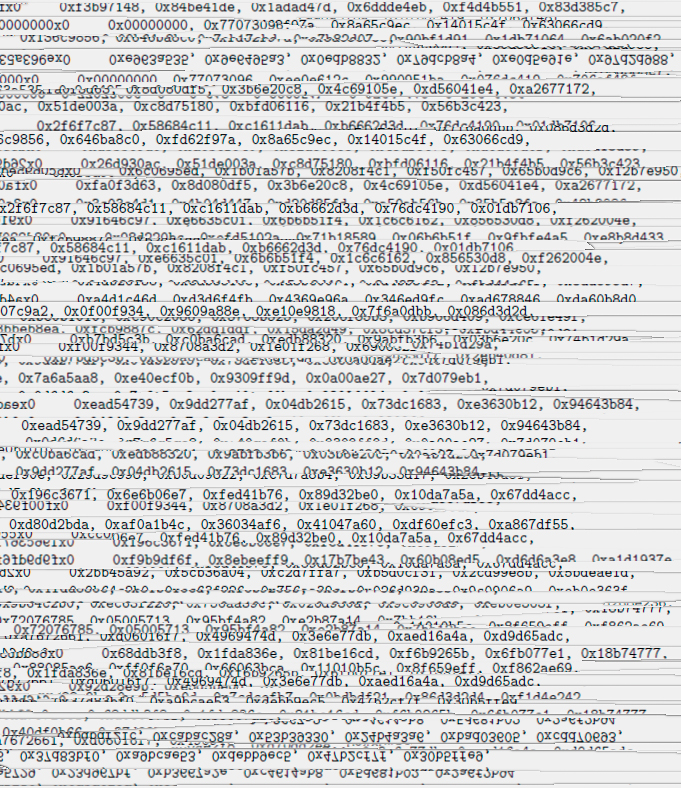
\includegraphics[scale=\FigScale]{cover.jpg}
\end{figure}

\bigskip

\hfill \huge \AUTHOR

\vspace*{\fill}
\end{center}

\newpage

\begin{center}
\vspace*{\fill}
\LARGE \TITLE

\vspace*{\fill}

\large \AUTHOR

\large \TT{<\EMAIL>}
\vspace*{\fill}
\vfill

\ccbyncnd

\textcopyright 2013-2014, \AUTHOR. 

\RU{Это произведение доступно по лицензии Creative Commons «Attribution-NonCommercial-NoDerivs» 
(«Атрибуция — Некоммерческое использование — Без производных произведений») 3.0 Непортированная. 
Чтобы увидеть копию этой лицензии, посетите}
\EN{This work is licensed under the Creative Commons Attribution-NonCommercial-NoDerivs 3.0 Unported License. 
To view a copy of this license, visit} \url{http://creativecommons.org/licenses/by-nc-nd/3.0/}.

\RU{Версия этого текста}\EN{Text version} ({\large \today}).

\RU{Возможно, более новая версии текста, а также англоязычная версия, также доступна по ссылке}
\EN{There is probably a newer version of this text, and Russian language version also accessible at} 
\href{http://go.yurichev.com/17009}{beginners.re}.
\ifdefined\ebook
\RU{Версия формата A4 так же доступна по ссылке.}
\EN{A4-format version is also available on the page.}
\else
\RU{Версия для электронных читалок так же доступна по ссылке.}
\EN{E-book reader version is also available on the page.}
\fi

\ifx\LITE\undefined
\RU{Существует также сокращенная LITE-версия (вводная), предназначенная для быстрого ознакомления
с основами reverse engineering}
\EN{There are also shortened LITE-version (introductory), intended to those who wants 
very quick introduction to reverse engineering basics}:
\href{http://go.yurichev.com/17358}{beginners.re}
\fi

\RU{Вы также можете подписаться на мой twitter для получения информации о новых версиях этого текста, 
и т.д: \TT{@yurichev}\footnote{\href{http://go.yurichev.com/17021}{twitter}}, 
либо подписаться на список рассылки}
\EN{You may also subscribe to my twitter, to get information about updates of this text, etc: 
\TT{@yurichev}\footnote{\href{http://go.yurichev.com/17021}{twitter}}
or to subscribe to mailing list}
\footnote{\href{http://go.yurichev.com/17020}{yurichev.com}}.

\RU{Обложка нарисована Андреем Нечаевским}\EN{The cover was made by Andy Nechaevsky}: \href{http://go.yurichev.com/17023}{facebook}.

\end{center}
\end{titlepage}
